% Section 3: Image selection and processing

\section{Image selection and processing}
\label{sec:image-selection-and-processing}


\subsection{Image selection}
\label{sec:image-selection}

Cassini observations were organized into observing campaigns. Each campaign was given a unique identifier (the observation name), which has the general format:

\begin{CodeBlock}
[INST]_[REV][TI]_[UNIQUENAME]_[PINST]
\end{CodeBlock}

where for the observations included in this bundle:

\begin{itemize}
\item INST is the abbreviation for the instrument being commanded (usually “ISS”)
\item REV is the rev (orbit) identifier, starting with 000 at Saturn orbit insertion and ending with 293 at the end of the mission. A few early revs are lettered instead of numbered; this bundle contains rev \code{00A}. Software that splits an observation name should treat REV as a fixed field of three characters and not assume it is an integer
\item TI is a 2-character target identifier: RA (A ring), RB (B ring), RF (F ring), RI (general rings), ST (star)
\item UNIQUENAME is a unique descriptor chosen by the observation creator, often containing acronyms such as “LP” for low phase, “HR” for high resolution, and “MOV” for movie. Some of the more common names:
\begin{itemize}
\item APOMOS* – Images taken at Cassini apoapse, often used to make large mosaics
\item AZSCN* – Azimuthal scan around the rings
\item *OCC – Stellar occultation
\item COMPLIT* – Radial composition scan on the lit side of the rings
\item EGAPMOVMP – Encke gap movie, medium phase
\item FMONITOR – F ring monitor; often an ISS rider on CIRS scans of the A and B rings
\item FMOVIE – Stared at a fixed inertial longitude to image F ring material passing through the field of view
\item FMOVIEEQX – F ring movie at Saturn equinox
\item FRSTRCHAN – Prometheus and F ring streamer-channel movie; tracks Prometheus and follows a small section of the F ring around one complete orbit
\item HIRESAFRG – High-resolution A ring outer edge
\item HIRESFRNG – High-resolution F ring
\item LATPHASE – Latitude and phase angle; wide range of sub-spacecraft latitude and solar phase angle
\item PROPRETRG – Re-targeting known “propeller” moons to track their orbits
\item SPK*, SPOKEMOV* – Spoke observation; stared at a ring ansa at regular intervals to watch B ring spokes move through the field of view
\item SUBM*, TDIFS*, TMAP* – Thermal observations by the Composite Infrared Spectrometer (CIRS); ISS rider
\item UR* – Ultraviolet Imaging Spectrograph (UVIS) ring stellar occultation; ISS rider
\end{itemize}
\item PINST indicates the name of the prime instrument if other than the ISS \zcite{(Knowles 2018)}. If PINST is not “PRIME”, then the ISS images were a ride-along on observations designed for the other instrument.
\end{itemize}
The complete set of $\sim$100,000 images containing the F ring was manually inspected for high-quality images.

In general, an image was included in our data set if:

\begin{enumerate}
\item It was a member of a series of images taken at different corotating longitudes that could be stitched together into a mosaic;
\item It was taken with the “clear” filters;
\item It was not corrupted or partially downloaded; and
\item Its best radial resolution at the F ring was no coarser than $\sim$80 km/pixel.
\end{enumerate}
However, due to the variation in image attributes and quality, the final determination of which images to include was necessarily subjective. For example:

\begin{itemize}
\item Some images were included that do not meet requirement \#1. If a single WAC image contained enough of the F ring to subjectively make a good mosaic by itself, it was included. Also, some image sequences were included where the camera followed a single corotating longitude as it traversed different inertial longitudes.
\item Some images were included that do not meet requirement \#4. These included the 42 “SPOKEMOV” mosaics taken at relatively low resolution by the WAC. While the reprojected images for these sequences are not of very high quality, the resulting mosaics are nevertheless sufficient for research, such as photometry, that does not require high-resolution analysis.
\end{itemize}
In total, 20,584 images were chosen for inclusion.

Image sequences were grouped under their original observation name converted to lowercase. In some cases, a single observation contained multiple distinct image sequences that would make different mosaics. In these cases, a unique numeric suffix was appended to the observation name.

The selected observations were divided into the classes described in the following sections. Every class except the default is indicated in the data archive by a comment in the mosaic PDS4 label and by a note in the global index file; Section~\ref{sec:the-global-index-files} lists the full set of notes.


\subsubsection{Standard inertial F movies}
\label{sec:standard-inertial-f-movies}

A standard “F movie” consists of a series of images taken while Cassini stared at approximately the same inertial longitude. The F ring rotated under the camera for some or all of a complete orbit, providing a partial or complete view of the entire longitudinal extent of the ring. Such observations are considered the default and are thus not marked with a special note.

It is important to realize that it was the F ring that was rotating, not the camera that was instantaneously observing different parts of the ring. The resulting image sequence and mosaic therefore do not provide a view of the F ring around its entire orbit. Instead, it provides repeated views of the F ring centered at (approximately) a single inertial longitude, and thus at a single true anomaly in its eccentric orbit. This can affect the interpretation of morphological features such as streamer-channels, which change shape throughout their orbit \zcite{(Attree et al. 2012, 2014; Beurle et al. 2010; French et al. 2014a; Murray et al. 2005, 2008)}.

An example of a standard mosaic is shown in Figure~\ref{fig:fmovie-mosaic}.


\subsubsection{M\#: Observations that are broken into chunks}
\label{sec:m-observations-that-are-broken-into-chunks}

Although Cassini observing campaigns are indicated by their observation name, sometimes a single campaign produced data that was more appropriately divided into multiple groups. In these cases, we produced multiple mosaics named after the observation name with a numerical suffix. The notes field in the index file (Section~\ref{sec:the-global-index-files}) includes “M1”, “M2”, “M3”, or “M4”, indicating how the different chunks are related to each other.


\paragraph{M1: Multiple contiguous observations of the same inertial longitude range}
\label{sec:m1-multiple-contiguous-observations-of-the-same}

In some cases, an observation stared at a single inertial longitude for more than a complete orbit of the F ring. In these cases, the observation was broken into multiple chunks, with each complete orbit of the F ring (and the final partial orbit, if there was one) used to create a separate mosaic. Such observations are noted in the index file with “M1”. The following mosaics have this flag, where a suffix list such as \code{\_\allowbreak{}1/\allowbreak{}2} stands for the separate mosaics \code{\_\allowbreak{}1} and \code{\_\allowbreak{}2}:

\begin{itemize}
\item \code{iss\_\allowbreak{}198ri\_\allowbreak{}spokemov005\_\allowbreak{}prime\_\allowbreak{}1/\allowbreak{}2}
\item \code{iss\_\allowbreak{}199ri\_\allowbreak{}spokemov002\_\allowbreak{}prime\_\allowbreak{}1/\allowbreak{}2}
\item \code{iss\_\allowbreak{}199ri\_\allowbreak{}spokemov003\_\allowbreak{}prime\_\allowbreak{}1/\allowbreak{}2/\allowbreak{}3}
\item \code{iss\_\allowbreak{}199ri\_\allowbreak{}spokemov004\_\allowbreak{}prime\_\allowbreak{}1/\allowbreak{}2}
\item \code{iss\_\allowbreak{}199ri\_\allowbreak{}spokemov006\_\allowbreak{}prime\_\allowbreak{}1/\allowbreak{}2/\allowbreak{}3}
\item \code{iss\_\allowbreak{}200ri\_\allowbreak{}spokemov004\_\allowbreak{}prime\_\allowbreak{}1/\allowbreak{}2/\allowbreak{}3}
\item \code{iss\_\allowbreak{}201ri\_\allowbreak{}spokemov001\_\allowbreak{}prime\_\allowbreak{}1/\allowbreak{}2}
\item \code{iss\_\allowbreak{}201ri\_\allowbreak{}spokemov009\_\allowbreak{}prime\_\allowbreak{}1/\allowbreak{}2}
\end{itemize}

\paragraph{M2: Pairs of observations taken at inertial longitudes 180° apart}
\label{sec:m2-pairs-of-observations-taken-at-inertial-longi}

Some observations were performed in pairs, where a particular range of corotating longitudes was observed at one inertial longitude, and then approximately the same range of corotating longitudes was observed at the inertial longitude roughly 180° away. Such pairs provide insight into how particles at the same corotating longitude are actually on slightly different orbits. These observations are divided into two chunks and noted with “M2”. The following mosaics have this flag:

\begin{itemize}
\item \code{iss\_\allowbreak{}085rf\_\allowbreak{}fmovie003\_\allowbreak{}prime\_\allowbreak{}1/\allowbreak{}2}
\item \code{iss\_\allowbreak{}094rf\_\allowbreak{}fmovie001\_\allowbreak{}prime\_\allowbreak{}1/\allowbreak{}2}
\item \code{iss\_\allowbreak{}112rf\_\allowbreak{}fmovie002\_\allowbreak{}prime\_\allowbreak{}1/\allowbreak{}2}
\item \code{iss\_\allowbreak{}173rf\_\allowbreak{}fmovie001\_\allowbreak{}prime\_\allowbreak{}1/\allowbreak{}2}
\item \code{iss\_\allowbreak{}174rf\_\allowbreak{}frstrchan001\_\allowbreak{}prime\_\allowbreak{}1/\allowbreak{}2}
\item \code{iss\_\allowbreak{}177rf\_\allowbreak{}fmovie001\_\allowbreak{}prime\_\allowbreak{}1/\allowbreak{}2}
\item \code{iss\_\allowbreak{}177rf\_\allowbreak{}frstrchan001\_\allowbreak{}prime\_\allowbreak{}1/\allowbreak{}2}
\item \code{iss\_\allowbreak{}183rf\_\allowbreak{}fmovie001\_\allowbreak{}prime\_\allowbreak{}1/\allowbreak{}2}
\item \code{iss\_\allowbreak{}193rf\_\allowbreak{}fmovie001\_\allowbreak{}prime\_\allowbreak{}1/\allowbreak{}2}
\item \code{iss\_\allowbreak{}194rf\_\allowbreak{}fmovie001\_\allowbreak{}prime\_\allowbreak{}1/\allowbreak{}2}
\item \code{iss\_\allowbreak{}198rf\_\allowbreak{}fmovie001\_\allowbreak{}prime\_\allowbreak{}1/\allowbreak{}2}
\item \code{iss\_\allowbreak{}201rf\_\allowbreak{}fmovie001\_\allowbreak{}prime\_\allowbreak{}1/\allowbreak{}2}
\item \code{iss\_\allowbreak{}202rf\_\allowbreak{}fmovie001\_\allowbreak{}prime\_\allowbreak{}1/\allowbreak{}2}
\item \code{iss\_\allowbreak{}203rf\_\allowbreak{}fmovie001\_\allowbreak{}prime\_\allowbreak{}1/\allowbreak{}2}
\item \code{iss\_\allowbreak{}208rf\_\allowbreak{}fmovie001\_\allowbreak{}prime\_\allowbreak{}1/\allowbreak{}2}
\item \code{iss\_\allowbreak{}208rf\_\allowbreak{}fmovie002\_\allowbreak{}prime\_\allowbreak{}1/\allowbreak{}2}
\item \code{iss\_\allowbreak{}209rf\_\allowbreak{}fmovie001\_\allowbreak{}prime\_\allowbreak{}1/\allowbreak{}2}
\item \code{iss\_\allowbreak{}212rf\_\allowbreak{}fmovie001\_\allowbreak{}prime\_\allowbreak{}1/\allowbreak{}2}
\item \code{iss\_\allowbreak{}232ri\_\allowbreak{}egapmovmp001\_\allowbreak{}prime\_\allowbreak{}1/\allowbreak{}2}
\item \code{iss\_\allowbreak{}233rf\_\allowbreak{}fmovie001\_\allowbreak{}prime\_\allowbreak{}1/\allowbreak{}2}
\item \code{iss\_\allowbreak{}235rf\_\allowbreak{}fmovie002\_\allowbreak{}prime\_\allowbreak{}1/\allowbreak{}2}
\item \code{iss\_\allowbreak{}239rf\_\allowbreak{}fmovie002\_\allowbreak{}prime\_\allowbreak{}1/\allowbreak{}2}
\item \code{iss\_\allowbreak{}243rf\_\allowbreak{}fmovie001\_\allowbreak{}prime\_\allowbreak{}1/\allowbreak{}2}
\item \code{iss\_\allowbreak{}256rf\_\allowbreak{}fmovie001\_\allowbreak{}prime\_\allowbreak{}1/\allowbreak{}2}
\item \code{iss\_\allowbreak{}276ri\_\allowbreak{}hiresafrg001\_\allowbreak{}prime\_\allowbreak{}1/\allowbreak{}2}
\end{itemize}
An example of such a pair of mosaics is shown in Figure~\ref{fig:paired-mosaics}.


\paragraph{M3: Multiple observations of the same corotating longitude range but different inertial longitude ranges}
\label{sec:m3-multiple-observations-of-the-same-corotating}

While standard “F movies” are taken by staring at a single inertial longitude in isolation, some observations were performed by taking multiple “F movies” in a row, each covering roughly the same range of corotating longitudes but at different inertial longitudes. These observations were split apart and are marked with “M3”. The following mosaics have this flag:

\begin{itemize}
\item \code{iss\_\allowbreak{}105ri\_\allowbreak{}tmapn45lp001\_\allowbreak{}cirs\_\allowbreak{}1–6}
\item \code{iss\_\allowbreak{}262rf\_\allowbreak{}fmovie001\_\allowbreak{}prime\_\allowbreak{}01–17}
\item \code{iss\_\allowbreak{}268rf\_\allowbreak{}fmovie001\_\allowbreak{}prime\_\allowbreak{}2–9}
\end{itemize}
An example is shown in Figure~\ref{fig:m3-mosaics}.


\paragraph{M4: Observations of different corotating and different inertial longitudes}
\label{sec:m4-observations-of-different-corotating-and-diff}

Finally, some observations follow neither a single corotating longitude nor a single inertial longitude. This is often the case for occultations. If both the ingress and egress occultations are imaged, the star’s position during ingress bears no fixed relation to its position during egress, nor to either the corotating or the inertial longitude. There are also some observations that are broken into different segments similar to “M3”, but each chunk observed both different corotating and inertial longitudes. These observations are marked with “M4”. The following mosaics have this flag:

\begin{itemize}
\item \code{iss\_\allowbreak{}185ri\_\allowbreak{}rhyaocc001\_\allowbreak{}vims\_\allowbreak{}1/\allowbreak{}2}
\item \code{iss\_\allowbreak{}191rf\_\allowbreak{}fmovie001\_\allowbreak{}prime\_\allowbreak{}1/\allowbreak{}2/\allowbreak{}3/\allowbreak{}4/\allowbreak{}5}
\item \code{iss\_\allowbreak{}201ri\_\allowbreak{}l2pupocc001\_\allowbreak{}vims\_\allowbreak{}1/\allowbreak{}2}
\item \code{iss\_\allowbreak{}206ri\_\allowbreak{}propretrg001\_\allowbreak{}prime\_\allowbreak{}1/\allowbreak{}2/\allowbreak{}3}
\item \code{iss\_\allowbreak{}239ri\_\allowbreak{}hiresafrg001\_\allowbreak{}prime\_\allowbreak{}1/\allowbreak{}2}
\item \code{iss\_\allowbreak{}253rf\_\allowbreak{}fmovie001\_\allowbreak{}prime\_\allowbreak{}1/\allowbreak{}2/\allowbreak{}3}
\item \code{iss\_\allowbreak{}268rf\_\allowbreak{}fmovie001\_\allowbreak{}prime\_\allowbreak{}1} (for this mosaic, all of the other chunks are marked with “M3”, but this chunk behaves differently)
\end{itemize}

\subsubsection{R: Follows one corotating longitude range with different inertial longitudes}
\label{sec:r-follows-one-corotating-longitude-range-with-di}

A small number of observations follow a single corotating longitude, taking one image at each inertial longitude. These are similar to the “M3” observations above, but contain such a small range of corotating longitudes in each image that it is not worth breaking them into separate mosaics. In these cases, a single mosaic is produced, but because the images overlap \textit{the mosaic is not particularly useful}. It is recommended instead to look at the corresponding reprojected images. These observations are marked with “R”. If a single observation is split into chunks, “R” may be paired with an appropriate “M” note. An example is shown in Figure~\ref{fig:r-reproj-imgs}. The following mosaics have this flag:

\begin{itemize}
\item \code{iss\_\allowbreak{}191rf\_\allowbreak{}fmovie001\_\allowbreak{}prime\_\allowbreak{}1/\allowbreak{}2/\allowbreak{}3/\allowbreak{}4/\allowbreak{}5}
\item \code{iss\_\allowbreak{}199rf\_\allowbreak{}fmovie002\_\allowbreak{}prime}
\item \code{iss\_\allowbreak{}256ri\_\allowbreak{}hiresafrg002\_\allowbreak{}prime}
\item \code{iss\_\allowbreak{}262rf\_\allowbreak{}fmovie001\_\allowbreak{}prime\_\allowbreak{}12}
\item \code{iss\_\allowbreak{}268rf\_\allowbreak{}fmovie001\_\allowbreak{}prime\_\allowbreak{}1}
\end{itemize}


\subsubsection{N: Neither inertial nor corotating}
\label{sec:n-neither-inertial-nor-corotating}

In a few cases, especially those involving wide-field views taken by the WAC, an observation can’t be classified as either inertial or corotating because the camera does not follow anything; it takes a single image, or a short series of images, covering large portions of the F ring. These cases are marked with “N”. An example is shown in Figure~\ref{fig:non-corot-mosaic}. The following mosaics have this flag:

\begin{itemize}
\item \code{iss\_\allowbreak{}007ri\_\allowbreak{}azscnloph001\_\allowbreak{}prime}
\item \code{iss\_\allowbreak{}039ri\_\allowbreak{}fmonitor002\_\allowbreak{}cirs}
\item \code{iss\_\allowbreak{}041ri\_\allowbreak{}fmonitor001\_\allowbreak{}cirs}
\item \code{iss\_\allowbreak{}043ri\_\allowbreak{}fmonitor001\_\allowbreak{}cirs}
\item \code{iss\_\allowbreak{}043ri\_\allowbreak{}fmonitor001\_\allowbreak{}prime}
\item \code{iss\_\allowbreak{}079ri\_\allowbreak{}fmonitor002\_\allowbreak{}prime}
\item \code{iss\_\allowbreak{}081ri\_\allowbreak{}fmonitor001\_\allowbreak{}prime}
\item \code{iss\_\allowbreak{}082ri\_\allowbreak{}fmonitor003\_\allowbreak{}prime}
\item \code{iss\_\allowbreak{}083ri\_\allowbreak{}fmonitor002\_\allowbreak{}prime}
\item \code{iss\_\allowbreak{}084ri\_\allowbreak{}fmonitor002\_\allowbreak{}prime}
\item \code{iss\_\allowbreak{}098ri\_\allowbreak{}tmapn30lp001\_\allowbreak{}cirs}
\item \code{iss\_\allowbreak{}100ri\_\allowbreak{}subms20lp001\_\allowbreak{}cirs}
\end{itemize}


\subsubsection{O: Occultation}
\label{sec:o-occultation}

Several observations were designed to monitor a stellar occultation of the F ring core. These observations continuously observed the position of the star as the F ring rotated. Since each image has the star in it, the mosaic may show the star multiple times. Like the “R” mosaics, these mosaics are \textit{not particularly useful by themselves} and it is recommended to look at the original reprojected images instead. Also, since these are “ride-along” observations where the Cassini Visible and Infrared Mapping Spectrometer (VIMS) or UVIS was the prime instrument measuring the photon flux, the ISS image sequences do not necessarily show the moment when the star was occulted by the F ring.

The observations \code{iss\_\allowbreak{}185ri\_\allowbreak{}rhyaocc001\_\allowbreak{}vims} and \code{iss\_\allowbreak{}201ri\_\allowbreak{}l2pupocc001\_\allowbreak{}vims} observed both the ingress and egress and thus are split into two chunks and also marked with “M4”.

The occultation observations are marked with “O”. The following mosaics have this flag, along with the star that each observation was pointed at:

\begin{itemize}
\item \code{iss\_\allowbreak{}172ri\_\allowbreak{}betpegocc001\_\allowbreak{}vims} — Scheat (Beta Pegasi)
\item \code{iss\_\allowbreak{}172st\_\allowbreak{}urgampeg001\_\allowbreak{}uvis} — Algenib (Gamma Pegasi)
\item \code{iss\_\allowbreak{}180ri\_\allowbreak{}rlyrocc001\_\allowbreak{}vims} — R Lyrae (13 Lyrae)
\item \code{iss\_\allowbreak{}180ri\_\allowbreak{}rcasocc001\_\allowbreak{}vims} — R Cassiopeiae
\item \code{iss\_\allowbreak{}185ri\_\allowbreak{}rhyaocc001\_\allowbreak{}vims\_\allowbreak{}1/\allowbreak{}2} — R Hydrae
\item \code{iss\_\allowbreak{}191ri\_\allowbreak{}rcasoccb001\_\allowbreak{}vims} — R Cassiopeiae
\item \code{iss\_\allowbreak{}194ri\_\allowbreak{}mucepocc001\_\allowbreak{}vims} — Herschel’s Garnet Star (Mu Cephei)
\item \code{iss\_\allowbreak{}196ri\_\allowbreak{}betandocc001\_\allowbreak{}vims} — Mirach (Beta Andromedae)
\item \code{iss\_\allowbreak{}197ri\_\allowbreak{}whyaocc001\_\allowbreak{}vims} — W Hydrae
\item \code{iss\_\allowbreak{}198ri\_\allowbreak{}rlyrocc001\_\allowbreak{}vims} — R Lyrae (13 Lyrae)
\item \code{iss\_\allowbreak{}201ri\_\allowbreak{}l2pupocc001\_\allowbreak{}vims\_\allowbreak{}1/\allowbreak{}2} — L2 Puppis
\item \code{iss\_\allowbreak{}205ri\_\allowbreak{}l2pupocc002\_\allowbreak{}vims} — L2 Puppis
\item \code{iss\_\allowbreak{}206ri\_\allowbreak{}l2pupocc002\_\allowbreak{}vims} — L2 Puppis
\end{itemize}

Each of these stars is named in a \code{Target\_\allowbreak{}Identification} block in the label of every data product belonging to its observation, and is linked there to the PDS context product for the star; the bundle and collection labels list the full set of stars observed.


\subsubsection{Reprojected images that were not used in a mosaic}
\label{sec:reprojected-images-not-used-in-a-mosaic}

For most observations, the reprojected images archived here are exactly those that contributed data to the observation’s mosaic. The “R” (Section~\ref{sec:r-follows-one-corotating-longitude-range-with-di}) and “O” (Section~\ref{sec:o-occultation}) observations are the exceptions. For these, the mosaic is of limited use and the reprojected images are the product of interest, so every reprojected image from the observation is archived, whether or not it supplied any data to the mosaic.

A reprojected image that did not contribute to the mosaic is not listed in the mosaic’s \code{OBSID\_\allowbreak{}mosaic[\_\allowbreak{}bkg\_\allowbreak{}sub]\_\allowbreak{}metadata\_\allowbreak{}src\_\allowbreak{}imgs.\allowbreak{}tab} file and is never referenced by the \code{image\_\allowbreak{}index} column of \code{OBSID\_\allowbreak{}mosaic[\_\allowbreak{}bkg\_\allowbreak{}sub]\_\allowbreak{}metadata\_\allowbreak{}params.\allowbreak{}tab} (Section~\ref{sec:data-mosaic-and-data-mosaic-bkg-sub}). The description in each reprojected image’s own label states which of the two cases applies.


\begin{figure}[tbp]
\centering
\noindent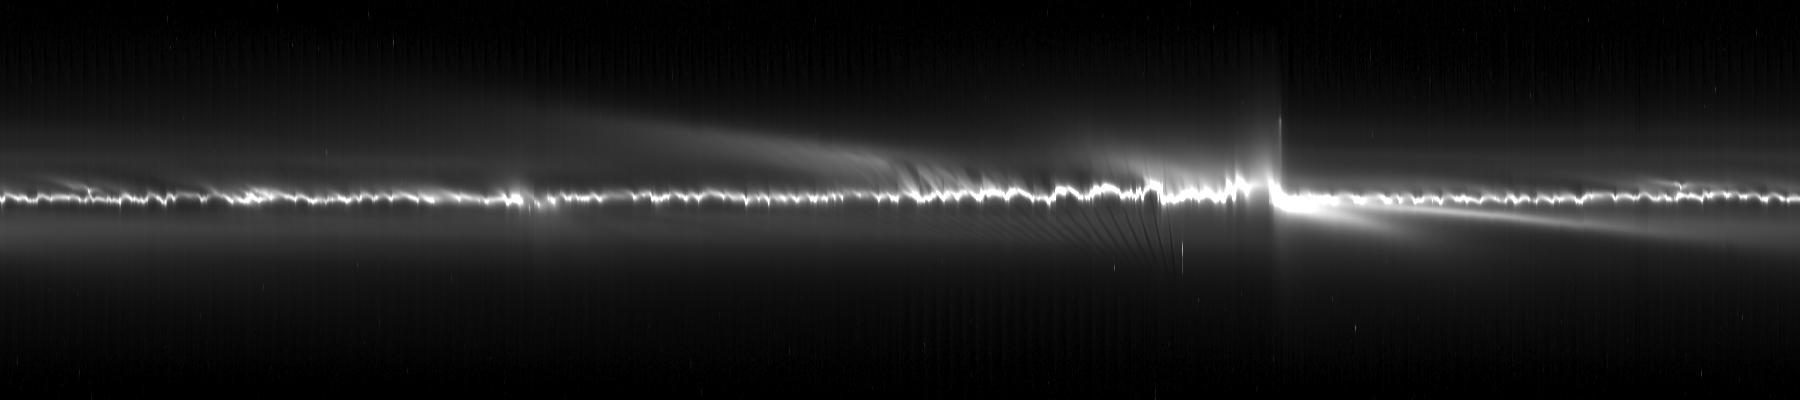
\includegraphics[width=\linewidth]{figures/fig1-fmovie-mosaic.png}
\caption{Mosaic of observation \code{iss\_\allowbreak{}039rf\_\allowbreak{}fmovie001\_\allowbreak{}vims}, a standard F movie taken as a rider on a VIMS-prime observation.}
\label{fig:fmovie-mosaic}
\end{figure}

\begin{figure}[tbp]
\centering
\noindent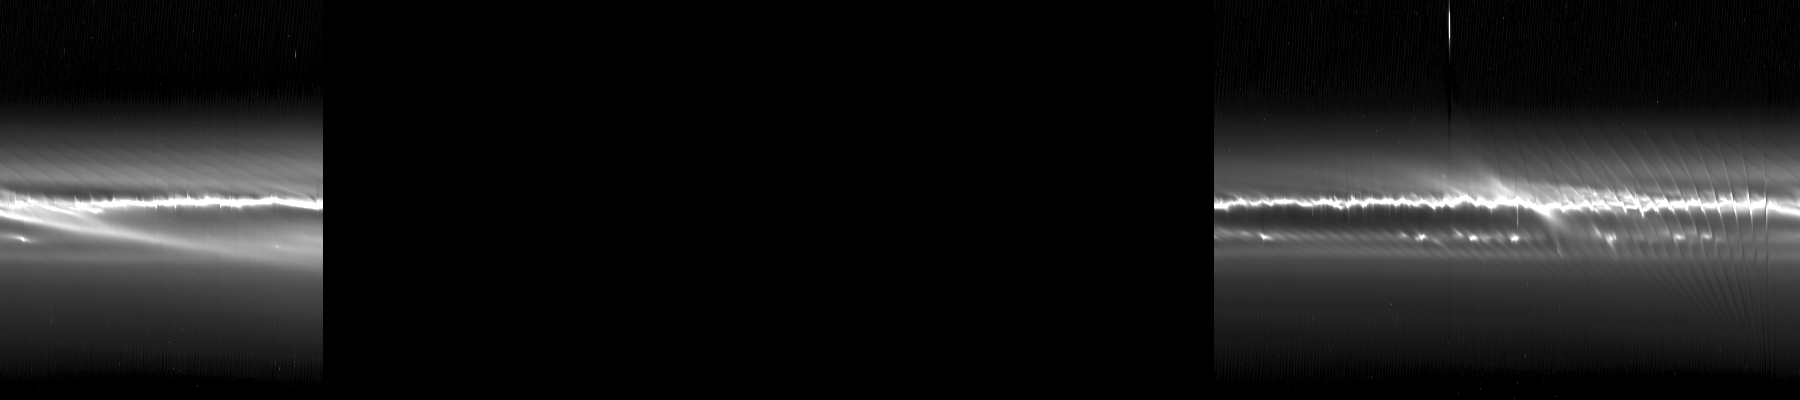
\includegraphics[width=\linewidth]{figures/fig2a-paired-mosaic-1.png}\\[2pt]
\noindent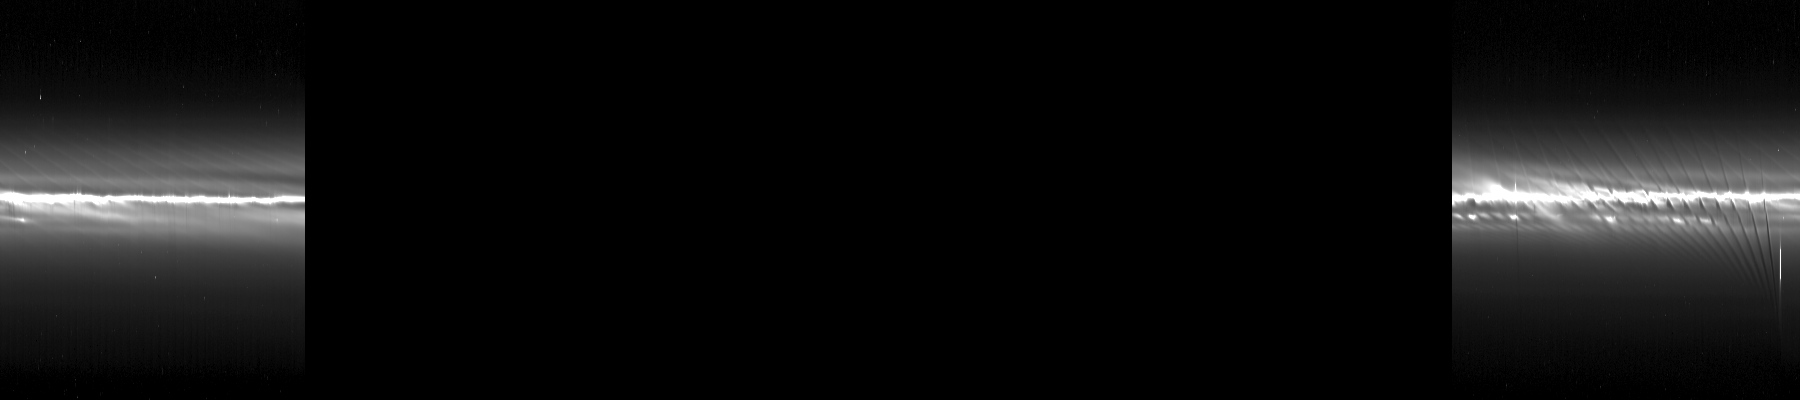
\includegraphics[width=\linewidth]{figures/fig2b-paired-mosaic-2.png}
\caption{Mosaics of observations \code{iss\_\allowbreak{}112rf\_\allowbreak{}fmovie002\_\allowbreak{}prime\_\allowbreak{}1} (top) and \code{iss\_\allowbreak{}112rf\_\allowbreak{}fmovie002\_\allowbreak{}prime\_\allowbreak{}2} (bottom). They cover approximately the same range of corotating longitudes but were taken at inertial longitudes roughly 180° apart. Morphological differences between the two are visible, giving potential insight into the orbits of the particles in these regions. (Flag M2.)}
\label{fig:paired-mosaics}
\end{figure}

\begin{figure}[tbp]
\centering
\noindent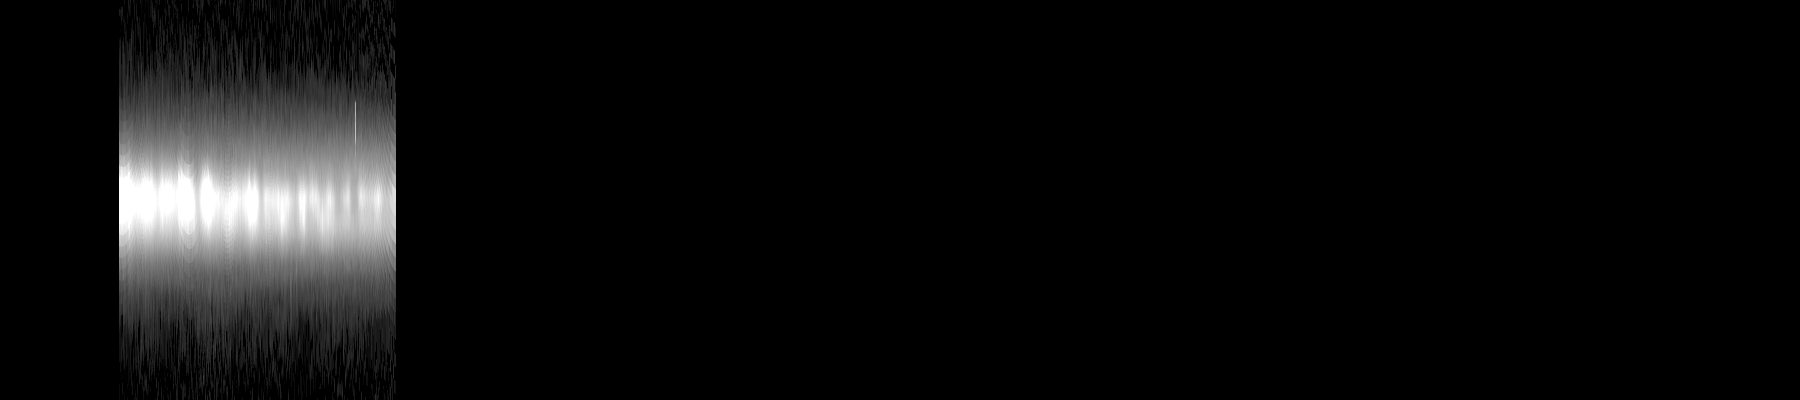
\includegraphics[width=\linewidth]{figures/fig3a-m3-mosaic-1.png}\\[2pt]
\noindent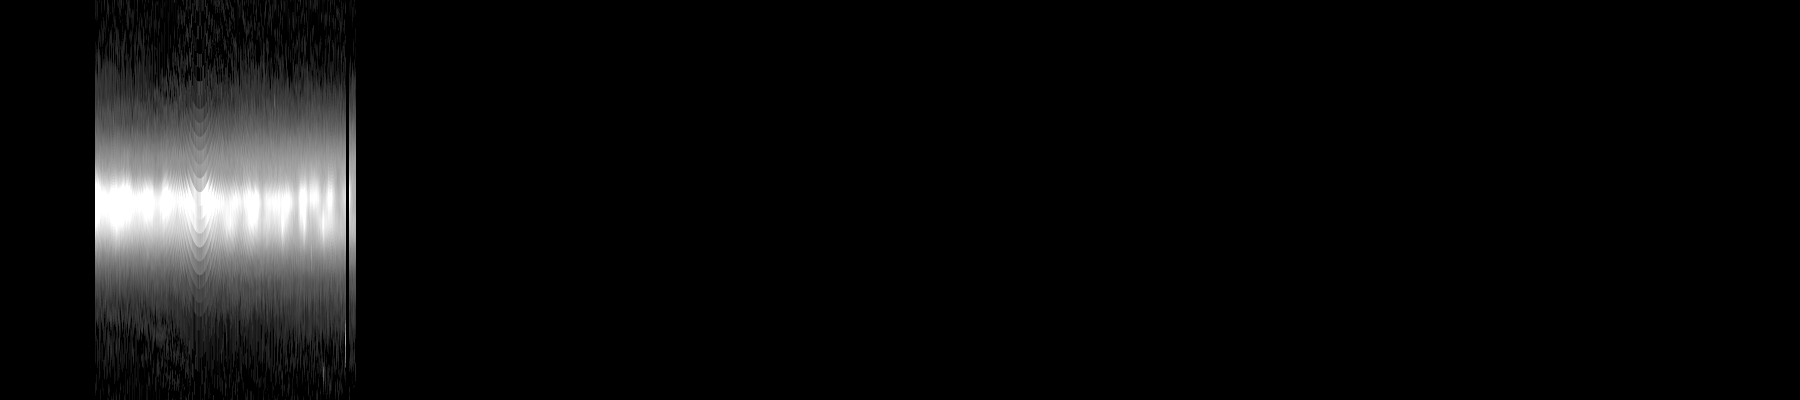
\includegraphics[width=\linewidth]{figures/fig3b-m3-mosaic-2.png}\\[2pt]
\noindent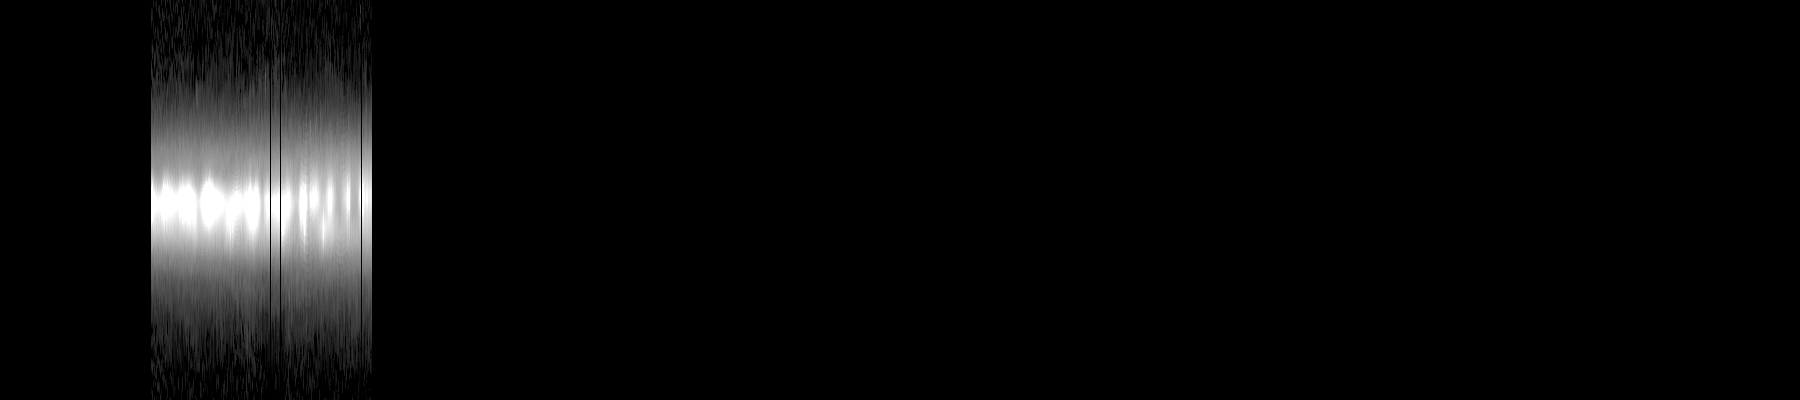
\includegraphics[width=\linewidth]{figures/fig3c-m3-mosaic-3.png}
\caption{A series of observations covering the same corotating longitudes but taken at successively increasing inertial longitudes. \code{iss\_\allowbreak{}105ri\_\allowbreak{}tmapn45lp001\_\allowbreak{}cirs\_\allowbreak{}1} (top) was taken at 78°–130°; \code{iss\_\allowbreak{}105ri\_\allowbreak{}tmapn45lp001\_\allowbreak{}cirs\_\allowbreak{}2} (middle) at 109°–154°; \code{iss\_\allowbreak{}105ri\_\allowbreak{}tmapn45lp001\_\allowbreak{}cirs\_\allowbreak{}3} (bottom) at 136°–186°. (Flag M3.)}
\label{fig:m3-mosaics}
\end{figure}

\begin{figure}[tbp]
\centering
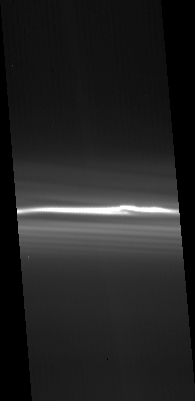
\includegraphics[width=0.327\linewidth]{figures/fig4a-reproj-img-1.png}
\hfill
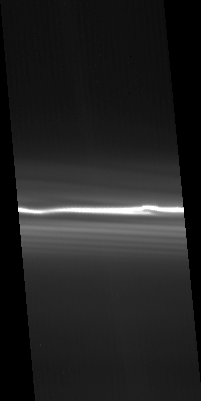
\includegraphics[width=0.327\linewidth]{figures/fig4b-reproj-img-2.png}
\hfill
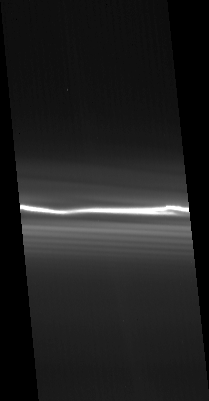
\includegraphics[width=0.327\linewidth]{figures/fig4c-reproj-img-3.png}
\caption{Three reprojected images from mosaic \code{iss\_\allowbreak{}191rf\_\allowbreak{}fmovie001\_\allowbreak{}prime\_\allowbreak{}1}, each covering approximately the same 4° range of corotating longitude. Source image index 0, \code{1748745661n} (left), was taken at inertial longitudes 5.7°–9.6°; index 4, \code{1748746261n} (middle), at 9.3°–13.3°; index 8, \code{1748746865n} (right), at 12.9°–17.1°. (Flag R.)}
\label{fig:r-reproj-imgs}
\end{figure}

\begin{figure}[tbp]
\centering
\noindent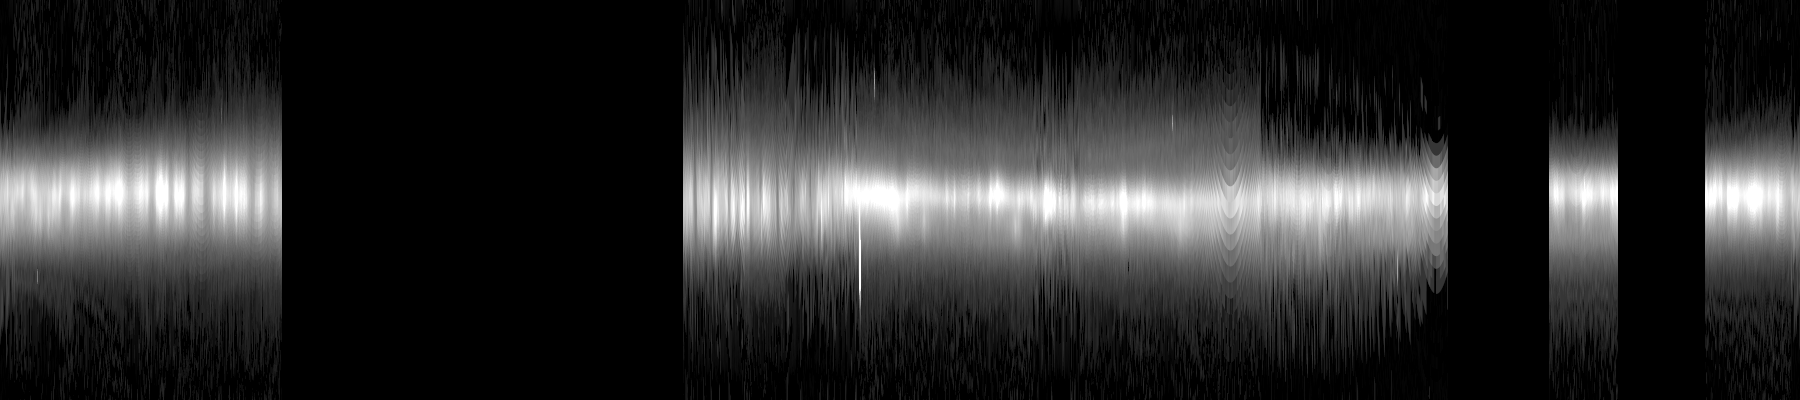
\includegraphics[width=\linewidth]{figures/fig5-non-corot-mosaic.png}
\caption{Non-inertial, non-corotating mosaic \code{iss\_\allowbreak{}098ri\_\allowbreak{}tmapn30lp001\_\allowbreak{}cirs}, which covers most of the full corotating range 0°–359.98°, taken from inertial longitudes 93°–309°. (Flag N.)}
\label{fig:non-corot-mosaic}
\end{figure}

\clearpage

\subsection{Calibration}
\label{sec:calibration}

Calibrated images were retrieved from the PDS Ring-Moon Systems Node archive\footnote{\href{https://pds-rings.seti.org/holdings/calibrated/COISS_2xxx/}{https://pds-rings.seti.org/holdings/calibrated/COISS\_\allowbreak{}2xxx/}}. Each image was calibrated by the Node using the CISSCAL 4.0 pipeline \zcite{(Knowles 2018)} into units of I/F\footnote{I/F is a dimensionless value that gives the ratio of the observed intensity to the incoming flux from the light source, assuming a perfect Lambert surface illuminated at normal incidence. See French et al. \zcite{(2012)} for more details.}. At the time of writing, the calibrated files are being migrated to the PDS4 standard, and they will be archived as collections within the \code{cassini\_\allowbreak{}iss\_\allowbreak{}cruise} and \code{cassini\_\allowbreak{}iss\_\allowbreak{}saturn} bundles.\footnote{\href{https://pds-rings.seti.org/pds4/bundles/cassini_iss}{https://pds-rings.seti.org/pds4/bundles/cassini\_\allowbreak{}iss}}


\subsection{Navigation}
\label{sec:navigation}

The spacecraft pointing information present in SPICE C kernels is known to have errors on the order of dozens of NAC pixels. Before processing each image, an automatic navigation procedure \zcite{(French et al. 2014b, 2016)} was performed that matched the image with features predicted to be present in it, such as stars and the edge of the A ring. Once a mosaic was created from a set of images, the quality of the navigation was evaluated by eye and, in some cases, the navigation of some images was manually adjusted for the best visual result. The (automatically or manually) adjusted C matrix for each image is reported in a supplemental file called \code{IMGID\_\allowbreak{}reproj\_\allowbreak{}img\_\allowbreak{}suppl.\allowbreak{}txt} in the \code{data\_\allowbreak{}reproj\_\allowbreak{}img} collection. See Section~\ref{sec:data-reproj-img}.

The outcome of that visual evaluation is recorded for each mosaic in the \code{nav\_\allowbreak{}quality} field of the mosaic label and the global index files (Section~\ref{sec:the-global-index-files}). The grade is subjective and describes the mosaic as a whole:

\begin{itemize}
\item \textbf{G} (good): the ring core runs continuously across the mosaic, with no visible radial step or tilt where one source image abuts the next.
\item \textbf{F} (fair): small radial steps or tilts are visible at some image boundaries, but the core is unambiguous at every longitude and photometry is not noticeably affected.
\item \textbf{P} (poor): at least one source image is misregistered enough to displace the core visibly. The mosaic remains usable for many purposes, but measurements at the affected longitudes should be treated with caution.
\end{itemize}

Because the grade covers the whole mosaic, a mosaic graded \textbf{F} or \textbf{P} may still contain a majority of well-navigated images.


\subsection{Reprojection}
\label{sec:reprojection}

Each calibrated image was converted to a reprojected image by mapping the pixels in the source image onto a two-dimensional grid with corotating longitude on the X axis and distance from the nominal F ring core (Δ\textit{r}) on the Y axis.


\subsubsection{F ring orbit}
\label{sec:f-ring-orbit}

Various orbital fits for the F ring core have been developed over time \zcite{(Albers et al. 2012; Cooper et al. 2013; Cuzzi et al. 2024)}. We use the orbit fit from Albers et al. \zcite{(2012)}, Table 3, fit 2, throughout:

\begin{equation*}
\begin{aligned}
n &= 581.964^{\circ}\,\mathrm{/day} & a &= 140{,}221.3\ \mathrm{km} & e &= 0.00235 \\
\varpi_{0} &= 24.2^{\circ} & \dot{\varpi} &= 2.70025^{\circ}\,\mathrm{/day} \\
\Omega_{0} &= 15.0^{\circ} & \dot{\Omega} &= -2.68778^{\circ}\,\mathrm{/day}
\end{aligned}
\end{equation*}

The angles $\varpi_{0}$ and $\Omega_{0}$ are the values at $\mathit{ET} = 0$, the J2000 epoch (2000-01-01T12:00:00 Barycentric Dynamical Time, TDB), where \textit{ET} is the ephemeris time SPICE reports; the rates $\dot{\varpi}$ and $\dot{\Omega}$ carry them forward to the time of each observation, as in the core radius formula below. This epoch is separate from the corotation epoch defined below, which is used only to relate corotating and inertial longitude.

Inertial ring longitude is measured from the reference direction — the ascending node of Saturn’s equatorial plane on the Earth’s mean equator of J2000 — in the direction of orbital motion along that plane to the ring’s ascending node, and thence along the ring plane.

Corotating longitude is based on a reference frame that rotates with the mean motion of the F ring. We use 2007-01-01T00:00:00Z as the epoch when corotating longitude and inertial longitude are equal. To convert from inertial to corotating longitude:

\begin{equation*}\mathit{corot} = \left(\mathit{inertial} - n\,\frac{\mathit{ET} - \mathit{epoch\_ET}}{86400}\right) \bmod 360\end{equation*}

and to convert from corotating to inertial longitude:

\begin{equation*}\mathit{inertial} = \left(\mathit{corot} + n\,\frac{\mathit{ET} - \mathit{epoch\_ET}}{86400}\right) \bmod 360\end{equation*}

where \textit{ET} is the ephemeris (SPICE) time of the image in seconds and \textit{epoch\_\allowbreak{}ET} is the corotating epoch in seconds, equal to 220881665.1839181.

Note that the choice of epoch is arbitrary, and when comparing absolute corotating longitudes from different sources it is important to convert them to a common reference frame. For example, Murray et al. \zcite{(2008)} used 2007-01-01T12:00:00Z and French et al. \zcite{(2012)} used 2004-01-01T12:00:00Z, while French et al. \zcite{(2014a)} used the same epoch adopted here.

To determine the radius of the F ring core, we use the standard formula:

\begin{equation*}r_{\mathrm{core}}=\frac{a(1-e^{2})}{1+e\cos\left(\lambda-\left(\varpi_{0}+\dot{\varpi}\frac{\mathit{ET}}{86400}\right)\right)}\end{equation*}

where \textit{λ} is the inertial longitude (converted from the corotating longitude as described above), so that the argument of the cosine is the true anomaly.


\subsubsection{Reprojection process}
\label{sec:reprojection-process}

The reprojection grid runs from 0° to 359.98° in steps of 0.02° ($\sim$49 km) for corotating longitude (18,000 pixels), and −1000 km to +1000 km in steps of 5 km for Δ\textit{r} (401 pixels). This gives an aspect ratio of roughly 10:1. For each corotating longitude, the radius is relative to the absolute radius of the core at the associated inertial longitude and time. This means that, while the core of the F ring varies in radius from 139,892 km to 140,551 km throughout its orbit, the core in the reprojected image will always look like an approximately straight line at $\Delta r = 0$, corresponding to Y = 200. Note that the odd number of pixels on the Y axis provides an equal number of radii on either side of the core, with the predicted core precisely in the center.

As the majority of reprojected images cover only a few degrees of corotating longitude, archiving files of the complete 18,000 × 401 grid would be extremely wasteful. As a result, the reprojected image data products are clipped on the X axis to the minimum and maximum corotating longitudes that contain valid data; see the associated label for information on these values. In the case where the extent of a reprojected image wraps around from 359.98° to 0°, the minimum corotating longitude is larger than the maximum corotating longitude, and the reprojected image is stored in two sections, first from the minimum corotating longitude to 359.98° and then from 0° to the maximum corotating longitude. See Section~\ref{sec:data-reproj-img} for the formulas that map a longitude to a column in this case. In all cases, if there is missing data within the remaining grid (either due to insufficient radial extent available in the source image, or discontinuous corotating longitudes), it is marked with the sentinel value −999.

During the reprojection process, several other parameters are computed for each corotating longitude, as the mean over that radial slice:

\begin{itemize}
\item Phase angle (°)
\item Emission angle (°)
\item Incidence angle (°)
\item Radial resolution (km/pixel)
\item Longitudinal resolution (°/pixel)
\end{itemize}
Following standard planetary ring practice, incidence and emission angles are measured from the ring-plane normal on the sunlit side. The incidence angle is therefore always below 90°, and an emission angle below 90° means the ring is being viewed from its lit side.

These values are reported in a table \code{IMGID\_\allowbreak{}reproj\_\allowbreak{}img\_\allowbreak{}metadata\_\allowbreak{}params.\allowbreak{}tab} (Section~\ref{sec:data-reproj-img}) that is associated with each reprojected image. Other parameters describing the orbits of the F ring, Prometheus, and Pandora at the time of the source image are included as well:

\begin{itemize}
\item Core Radius (distance from Saturn in km, computed using the formula above)
\item Longitude of Ascending Node (°)
\item Longitude of Pericenter (°)
\item True Anomaly (°)
\item Corotating Longitude of Prometheus (°) in the same corotating frame used for the F ring
\item Radius (distance from Saturn) of Prometheus (km)
\item Corotating Longitude of Pandora (°) in the same corotating frame used for the F ring
\item Radius (distance from Saturn) of Pandora (km)
\end{itemize}
The positions of Prometheus and Pandora were computed with SPICE, taking the satellite positions from the Saturn system ephemeris \code{sat393.\allowbreak{}bsp}, planetary positions from \code{de438.\allowbreak{}bsp}, and the ring-plane orientation from the planetary constants kernel \code{pck00010\_\allowbreak{}edit\_\allowbreak{}v01.\allowbreak{}tpc}. The metakernel archived in this bundle’s \code{spice\_\allowbreak{}kernels} collection (Section~\ref{sec:the-spice-kernels-directory}) lists every kernel used anywhere in the production of this bundle, which is a larger set than these three.

Mean, minimum, and maximum values for many of these parameters are included in the label for each reprojected image as well. See Section~\ref{sec:reprojected-image-and-mosaic-metadata-params} for a complete list of the metadata parameters provided.


\subsection{Mosaic creation}
\label{sec:mosaic-creation}

Mosaics were created by stitching together one or more reprojected images. The resulting grid for a mosaic is the same 18,000 × 401 pixel grid as used for each reprojected image (Section~\ref{sec:reprojection}). For each corotating longitude in the mosaic, the entire radial stripe is taken from a single image. The image is chosen first based on which image has the most valid pixels at that corotating longitude; when there is a tie, the image with the smallest mean radial resolution is used. This guarantees that the resulting mosaic will have the most data and the highest resolution possible, but does not guarantee that the selected reprojected images will change monotonically with corotating longitude. This can result in a slight temporal “blurring” across small ranges of corotating longitude.

As with reprojected images, several parameters are stored for each corotating longitude and provided in a table file \code{OBSID\_\allowbreak{}mosaic\_\allowbreak{}metadata\_\allowbreak{}params.\allowbreak{}tab} (Section~\ref{sec:data-mosaic-and-data-mosaic-bkg-sub}) associated with each mosaic:

\begin{itemize}
\item Source reprojected image number
\item SPICE ET of source image
\item Mean phase angle (°)
\item Mean emission angle (°)
\item Incidence angle (°)
\item Mean radial resolution (km/pixel)
\item Mean longitudinal resolution (°/pixel)
\item Core Radius (distance from Saturn in km, computed using the formula above)
\item Longitude of Ascending Node (°)
\item Longitude of Pericenter (°)
\item True Anomaly (°)
\item Corotating Longitude of Prometheus (°) in the same corotating frame used for the F ring
\item Radius (distance from Saturn) of Prometheus (km)
\item Corotating Longitude of Pandora (°) in the same corotating frame used for the F ring
\item Radius (distance from Saturn) of Pandora (km)
\end{itemize}
Mean, minimum, and maximum values for many of these parameters are included in the label for each mosaic as well. See Section~\ref{sec:reprojected-image-and-mosaic-metadata-params} for a complete list of the metadata parameters provided.


\subsection{Background modeling}
\label{sec:background-modeling}

The final step in the data production pipeline is modeling and subtracting the background gradient for each mosaic. The background gradient is modeled separately for each corotating longitude using a linear function. Regions normally consisting of the innermost 50 rows ($\Delta r$ = −1000 to −755 km) and the outermost 51 rows ($\Delta r$ = +750 to +1000 km) are used to fit a linear model, which is then subtracted from the complete 401-row radial slice. When creating the model, pixel values that are statistically anomalous compared to nearby longitudes are automatically masked. This removes stars, Prometheus and Pandora, and bad pixels from the background model computation. In some cases, the standard range of 50 pixels on each side is not appropriate. Reasons include large objects such as Prometheus covering the entire 50-row range, the reprojected source images not providing data for the entire radial range (which would require the background margins to be increased in size), and very low-resolution images where the F ring bleeds over into the background region (which would require background margins to be reduced). Such determinations were made through careful examination of each mosaic and the extent of the background margin was manually adjusted as needed. Whenever possible, the new margins were chosen to have minimal effect on computation of equivalent width.\footnote{Equivalent width is a photometric value that integrates the brightness of a radial slice, taking into account the resolution of the image.} The chosen margins are reported in the label for each background-subtracted mosaic and in the \code{bkgnd\_\allowbreak{}lower\_\allowbreak{}limit} and \code{bkgnd\_\allowbreak{}upper\_\allowbreak{}limit} fields of the global index file (Section~\ref{sec:the-global-index-files}). Both are signed values of Δ\textit{r} in km, so that the interior background region runs from −1000 km out to \code{bkgnd\_\allowbreak{}lower\_\allowbreak{}limit} (normally −750 km) and the exterior region runs from \code{bkgnd\_\allowbreak{}upper\_\allowbreak{}limit} (normally +750 km) out to +1000 km.

In cases where, even after adjusting the margins, there was insufficient radial data to create a background model for some longitudes, those longitudes were marked as invalid and deleted from the background-subtracted mosaic. As a result, the background-subtracted mosaic may have fewer (and sometimes substantially fewer) valid longitudes than the original mosaic. An example is shown in Figure~\ref{fig:bkg-sub-mosaic}.

The model is fit to noisy data, so subtracting it leaves the background regions scattered about zero. Roughly half of the pixels away from the ring in a background-subtracted mosaic are consequently negative. This is expected. Keep these values instead of clipping them at zero; discarding the negative half of the noise biases any integral over a radial slice, equivalent width included.

Each background-subtracted mosaic was inspected and the result recorded in the \code{bkgnd\_\allowbreak{}quality} field of the label and the global index file (Section~\ref{sec:the-global-index-files}). Like \code{nav\_\allowbreak{}quality} (Section~\ref{sec:navigation}), the grade is subjective:

\begin{itemize}
\item \textbf{G} (good): the regions away from the ring are flat after subtraction at essentially all longitudes.
\item \textbf{F} (fair): a residual gradient or offset remains at some longitudes, small enough that equivalent widths are still usable.
\item \textbf{P} (poor): the model is visibly wrong over a substantial range of longitudes, usually because too little background data was available or because the F ring dust sheet extends into the background region.
\end{itemize}

\begin{figure}[tbp]
\centering
\noindent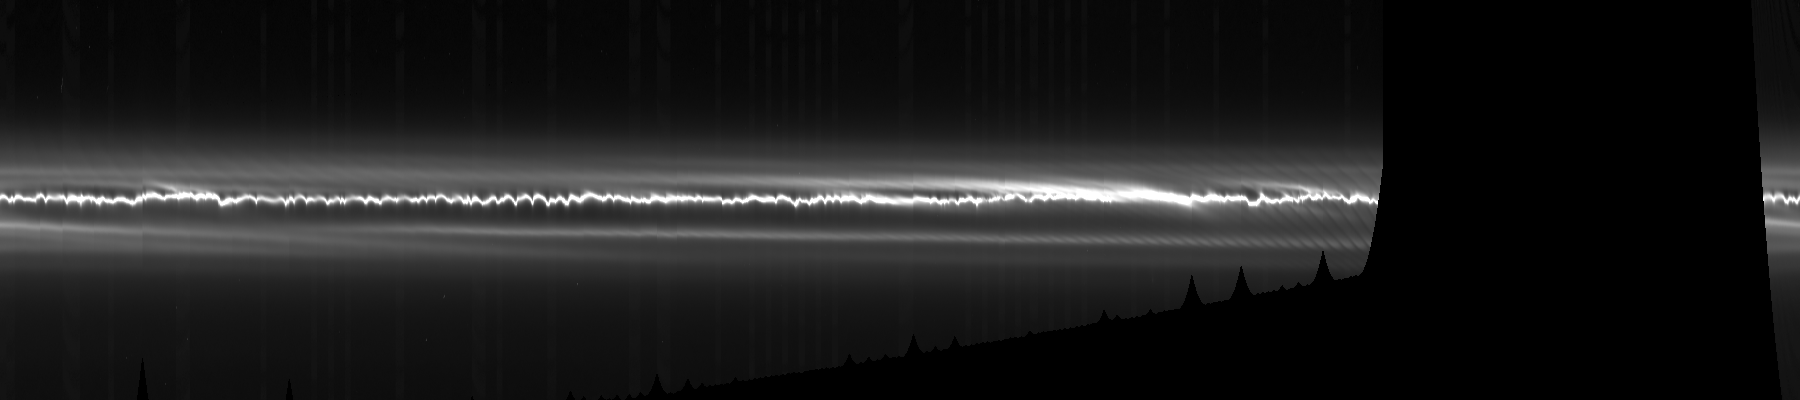
\includegraphics[width=\linewidth]{figures/fig6a-mosaic-original.png}\\[2pt]
\noindent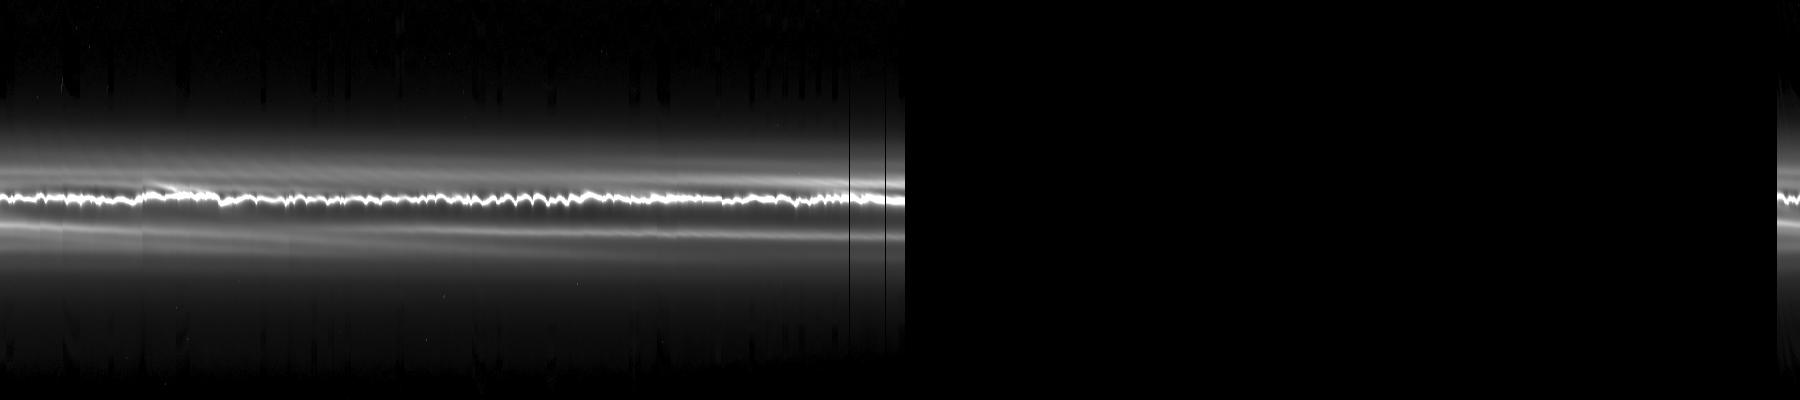
\includegraphics[width=\linewidth]{figures/fig6b-mosaic-bkg-sub.png}
\caption{Original mosaic iss\_\allowbreak{}007ri\_\allowbreak{}hpmrdfmov001\_\allowbreak{}prime (top) and associated background-subtracted mosaic (bottom). The lack of some data in the original mosaic (to the lower left of the large blank area) prevents the creation of a background model for those longitudes, resulting in a background-subtracted mosaic with substantially fewer valid longitudes.}
\label{fig:bkg-sub-mosaic}
\end{figure}
